\chapter{Estructura cristalina}

Las sustancias cristalinas se caracterizan por una periodicidad espacial perfecta, que facilita enormemente la tarea de comprender y calcular sus propiedades físicas. Las sustancias cristalinas se encuentran comúnmente en forma de policristales (aglomerados de pequeñas cristales orientados desordenadamenet llamads cristalitos o granos). Existe una categoría importante de sólidos, que no se tratará aquí denominados amorfos, como el vidrio común  y muchos polímeros, que no pertenecen a los sólidos cristalinos, pues aunque poseen cierto ordden de corto alcance carecen del orden de largo alcance característico de los critales.

\section{Conceptos básicos}

En esta sección introduciremos las definiciones más importantes que usaremos a lo largo del tema. \\

\begin{definition}[{\bf Red}]
    Cojunto de puntos discretos del espacio con vectores posición dados por la combinación lineal: 

    \begin{equation}
        \rn = u_1 \an_1 + u_2 \an_2 + u_3 \an_3 \label{Ec:01-01-01}
    \end{equation}
    donde los $u_i$ barren {\it todos} los enteros. Los $\an_i$ se denominan {\it vectores base primitivos}.
\end{definition}

\begin{definition}[{\bf Base atómica}]
    conjunto de átomos que se asocia a todos y cada uno de los puntos de la red.
\end{definition}

\begin{definition}[{\bf Estructura cristalina o cristal}]
    Es la combinación red+base atómica. Un ejemplo en 2D sería el representado por la figura.
\end{definition}

\begin{definition}[{\bf Celda unitaria primitiva}]
    Es un volumen del espacio que por traslaciones en vectores de la red cube todo el espacio (sin solapamientos). Una posible forma de construirla es por el paralepípedo definido por los vectores base primitivos.    
\end{definition}

\begin{definition}[{\bf Vectores base y celdas no primitivas}]
    Vectores base {\it no primitivos}: son aquellos que generan la red por combinaciones lineales de la forma \ref{Ec:01-01-01} pero donde los $u_i$ toman también valores no enteros. Un ejemplo es la celda cuadrada centrada que se muestra en la figura . Las celdas (unitarias) no primitivas correspondientes son simepre de mayor volumen que las primitivas por tener asociado más de un punto de red. Para algunos propósitos (por ejemplo, la {\it indexación} de máximos de difracción de rayos x que se verá en el Capitulo \ref{Ch:02}) la combinación red+base puede variarse, aunque sea a costa de aumentar el número de átomos de la base. La figura es un ejemplo: la estructura se puede describir como una red oblicua con base de un sólo círculo o como una red cuadrada con base de dos círculos (uno en el vértice y otro en el centro de la celda cuadrada).
\end{definition}

\begin{definition}[{\bf Primeras consecuencias}]
    Para una red existe más de una elección de vectores base primitivos, como se muestra en la figura . Todas las celdas primitivas tienen el mismo volumen pues tienen asociado uno y sólo un punto de red. Todos los puntos de una red son indistinguibles en el sentido de que la red {\it se ve} igual desde cualquiera de sus puntos. También se puede decir que es invariante por traslacciones de vectores de red (\it{simetría de traslación}).          
\end{definition}

\begin{definition}[{\bf Otras simetrías}]
    Invaria por {\it inversión} ($\Rn \rightarrow - \Rn$), {\it eje de rotación} de orden $n$ (invariancia por giro del ángulo $2\pi/n$ alrededor del eje), {\it planos de simetría, centros de inversión}...    
\end{definition}

\begin{definition}[{\bf Número de coordinación}]
    Es la número de vecinos más próximos (misma distancia) a un punto cualquiera de la red. La misma noción se aplica a átomos cuando se trata de cristales.
\end{definition}

\begin{definition}[{\bf Celda de Wigner-Seitz}]
    Se construye de la siguiente forma: trazar segmentos que concecntan a un punto dado de la red con todos sus vecinos próximos; trazar los planos mediatrices a dichas líneas. La región así encerrada (poliedro en 3D, polígono en 2D) es la celda de Wigner-Seitz. Ver el ejemplo ·D de la Figura  . La celda de Wigner-Seitz es primitva y contiene todas las simetrías de la red.    
\end{definition}

\begin{figure}[h!] \centering
    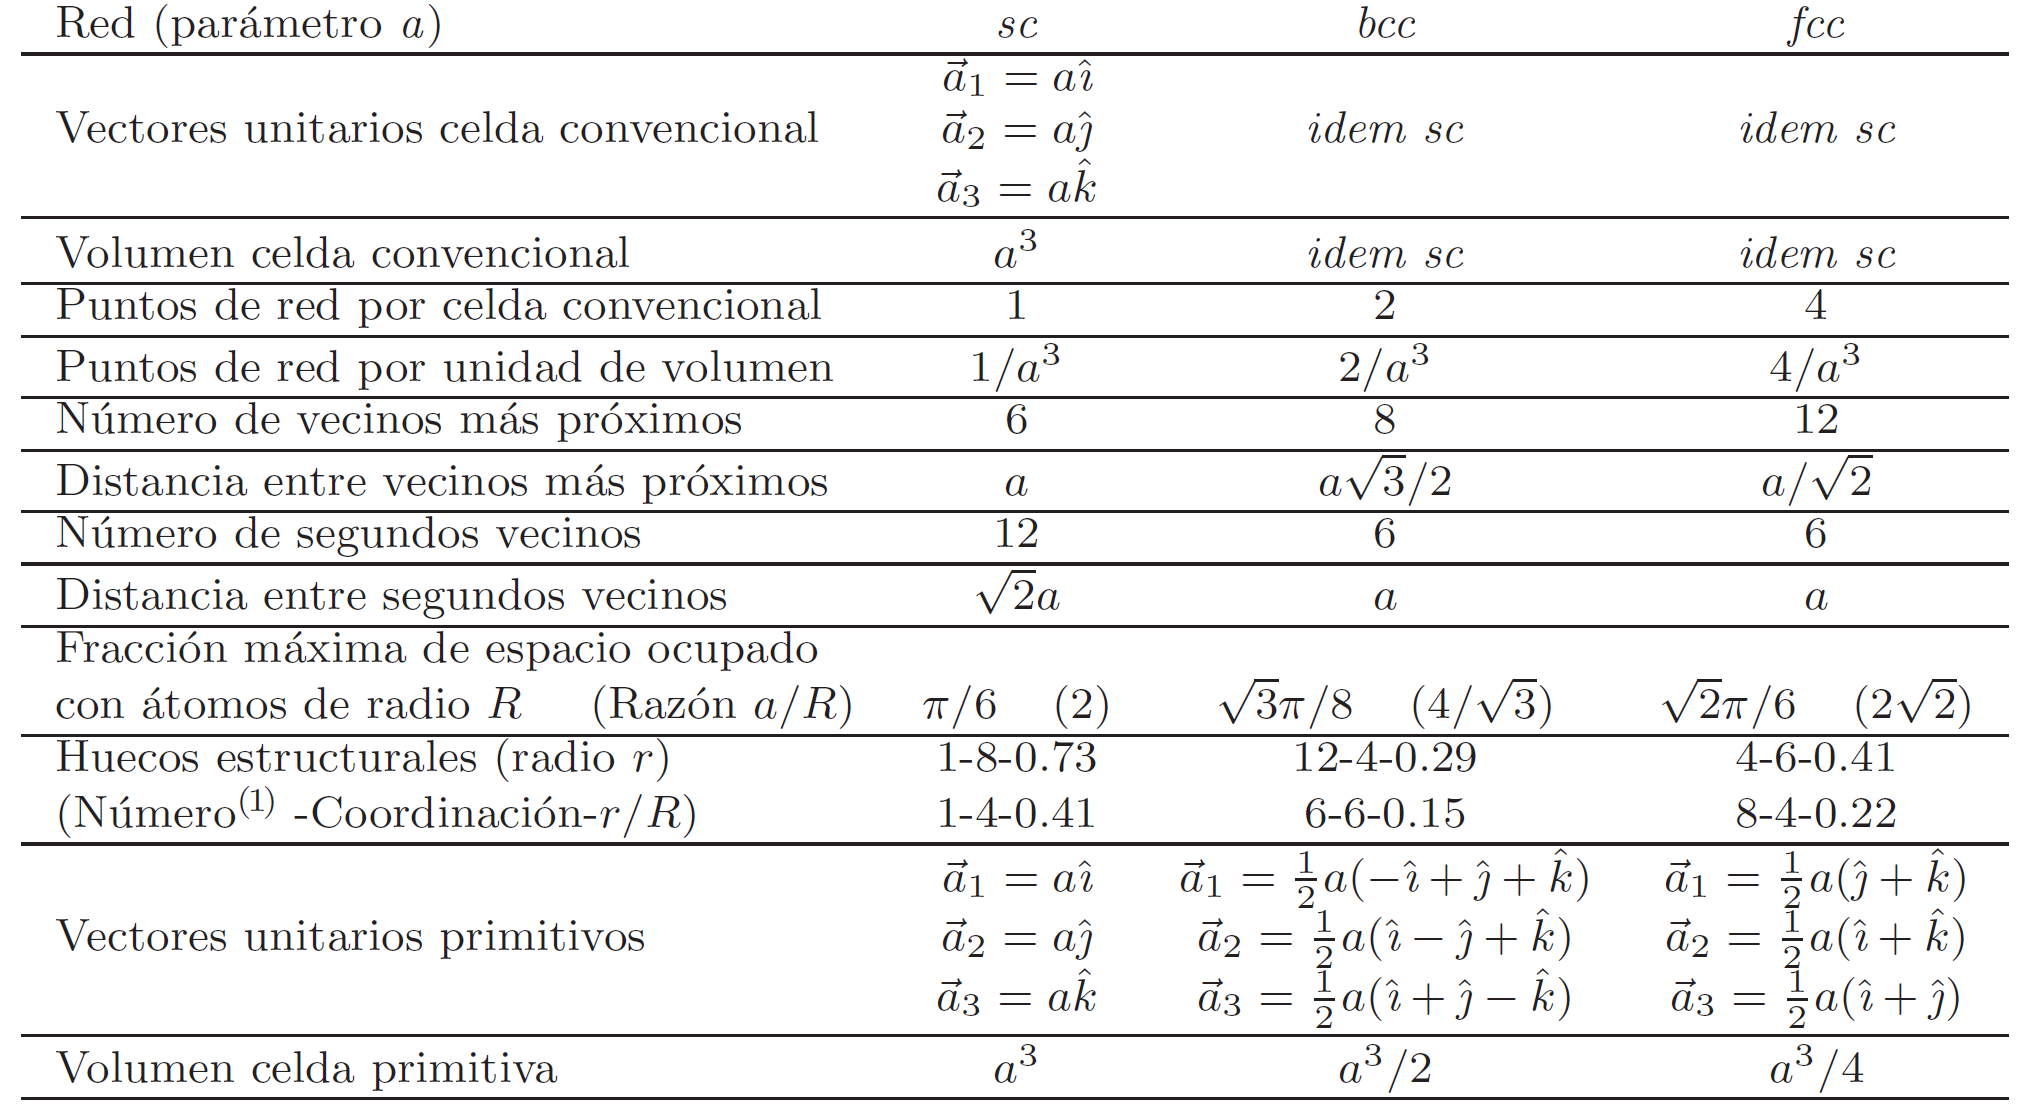
\includegraphics[scale=1]{.\Ch_01\datos.png}
\end{figure}

